%! Author = sbbfti
%! Date = 10/06/2020
\section{Results and Discussion}\label{sec:results}

\subsection{\ac{db2} overview}\label{subsec:comfort-db-overview}
While the \ac{db2} contains \var{entries_db_all} data points, only \var{entries_db_used} entries met the inclusion criteria listed in the Methodology section.
The distribution of the six input variables used to calculate the PMV indices is visualized in Figure~\ref{fig:dist_input_data} in which we excluded the data points below or above the 2.5th and 97.5th percentiles, respectively.
\begin{figure*}[htb!]
    \centering
    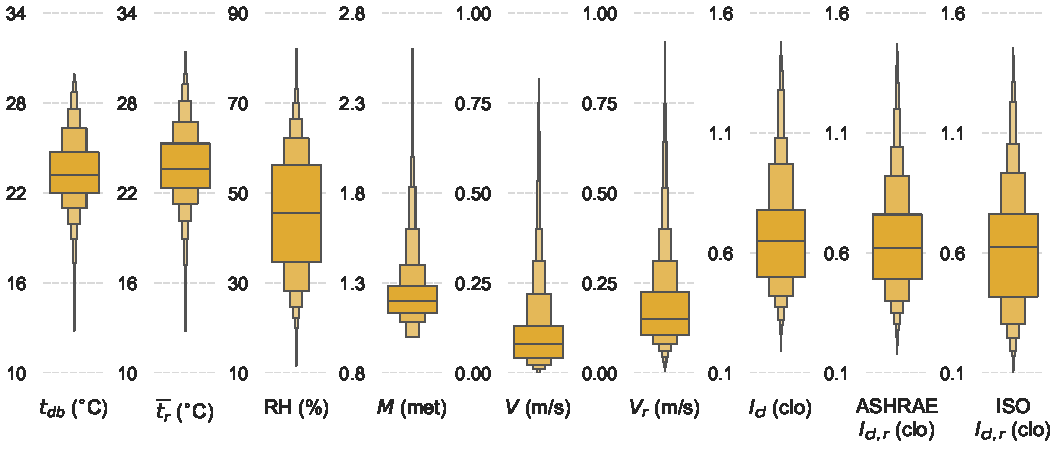
\includegraphics[width=\textwidth]{figures/dist_input_data}
    \caption{Distribution of the input variables used to calculate the \ac{pmv} and \ac{pmv-ce} values.
    We did not plot data points below or above the 2.5th and 97.5th percentiles, respectively.
    The data are shown using boxen plots (letter-value plots).
    They depict the median as the center-line and each successive level outward contains half of the remaining data.}
    \label{fig:dist_input_data}
\end{figure*}
The input data distributions are far from uniformity (equal density) across the Standards' applicability ranges.
We were not able to determine the accuracy of the \ac{pmv} and \ac{pmv-ce} formulations for inputs that were lower than the 2.5th and 97.5th percentiles, since we only had a limited number of data points beyond those values.
For example, only 2.5\% of the available dataset had a \ac{tdb} $\leq$ than \var{ta_95_perc_min}, this may consequently be an issue since both thermal comfort Standards' applicability limits extend to \qty{10}{\celsius}.
This can be explained by the fact that only a few buildings in the world operate at \ac{tdb} lower than this value.
This is because an indoor \ac{tdb} lower than \var{ta_95_perc_min} would be deemed to be unsatisfactory by a great number of occupants~\cite{iso7730}.
This lack of data in the \ac{db2} is particularly relevant for \ac{v}.
The \ac{pmv} and \ac{pmv-ce} only differ when the value of \ac{v} $\geq$ \qty{0.1}{\m\per\s}, however, the median value in the \ac{db2} was \qty{0.08}{\m\per\s} suggesting that most of the data points were collected in buildings with low air movement.
Consequently, we could not reliably test the accuracy of the \ac{pmv} formulations for values of \ac{v} $\geq$ \var{v_95_perc_max}.

Figure~\ref{fig:dist_other_data} shows the distribution of age, height, weight, and running mean outdoor temperature.
Less than half (\num{23300}) of the total entries have information about the participant's sex and are almost equally distributed among males \qty{52}{\percent} and females.
Ages are not normally distributed, the same is true for the running mean outdoor temperature.
About half of the participants (\qty{52}{\percent}) were aged between \num{20} and \num{35} years old, and only \qty{2.5}{\percent} were older than 60.
This limits our analysis to young adults and does not allow us to determine the accuracy of the \ac{pmv} and \ac{pmv-ce} models in predicting thermal sensation for children or older adults.
The \ac{db2} does not contain information about the health status of the participants.
Approximately \qty{56}{\percent} of the running mean outdoor temperature values where between \qtyrange{10}{25}{\celsius}.
\begin{figure*}[htb!]
    \centering
    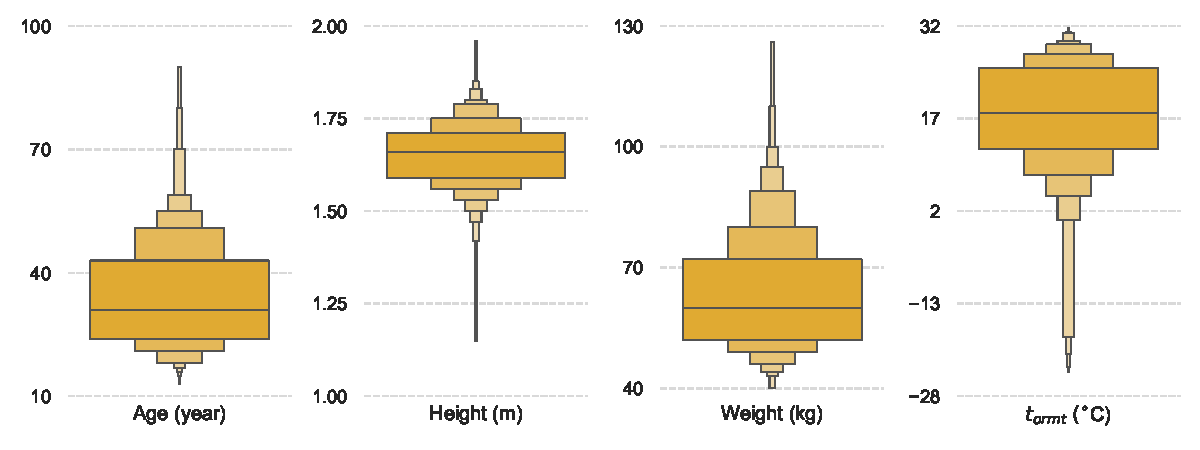
\includegraphics[width=\textwidth]{figures/dist_other_data}
    \caption{Distribution of age, height, weight, and running mean outdoor temperature.
    The data are grouped by sex.
    The text in blue is showing the 2.5th, 50th (median), and 97.5th percentiles.}
    \label{fig:dist_other_data}
\end{figure*}
The percentage of \ac{tpv} grouped by each \ac{tsv} is shown on the left side of Figure~\ref{fig:bar_plot_tp_by_ts}.
Only \var{entries_with_tp} entries had information about both \ac{tsv} and \ac{tpv}.
Thus, on the right, we show a bar chart depicting the distribution of all the \ac{tsv} votes, we analyzed in the paper.
The \ac{tsv} is unbalanced. 
Approximately \var{perc_tsv_neutral} of all the entries have a \ac{tsv} of `Neutral'.
While less than \var{perc_tsv_hot} of the total sample of participants reported to be either `Hot' or `Cold'.
\begin{figure*}[htb!]
    \centering
    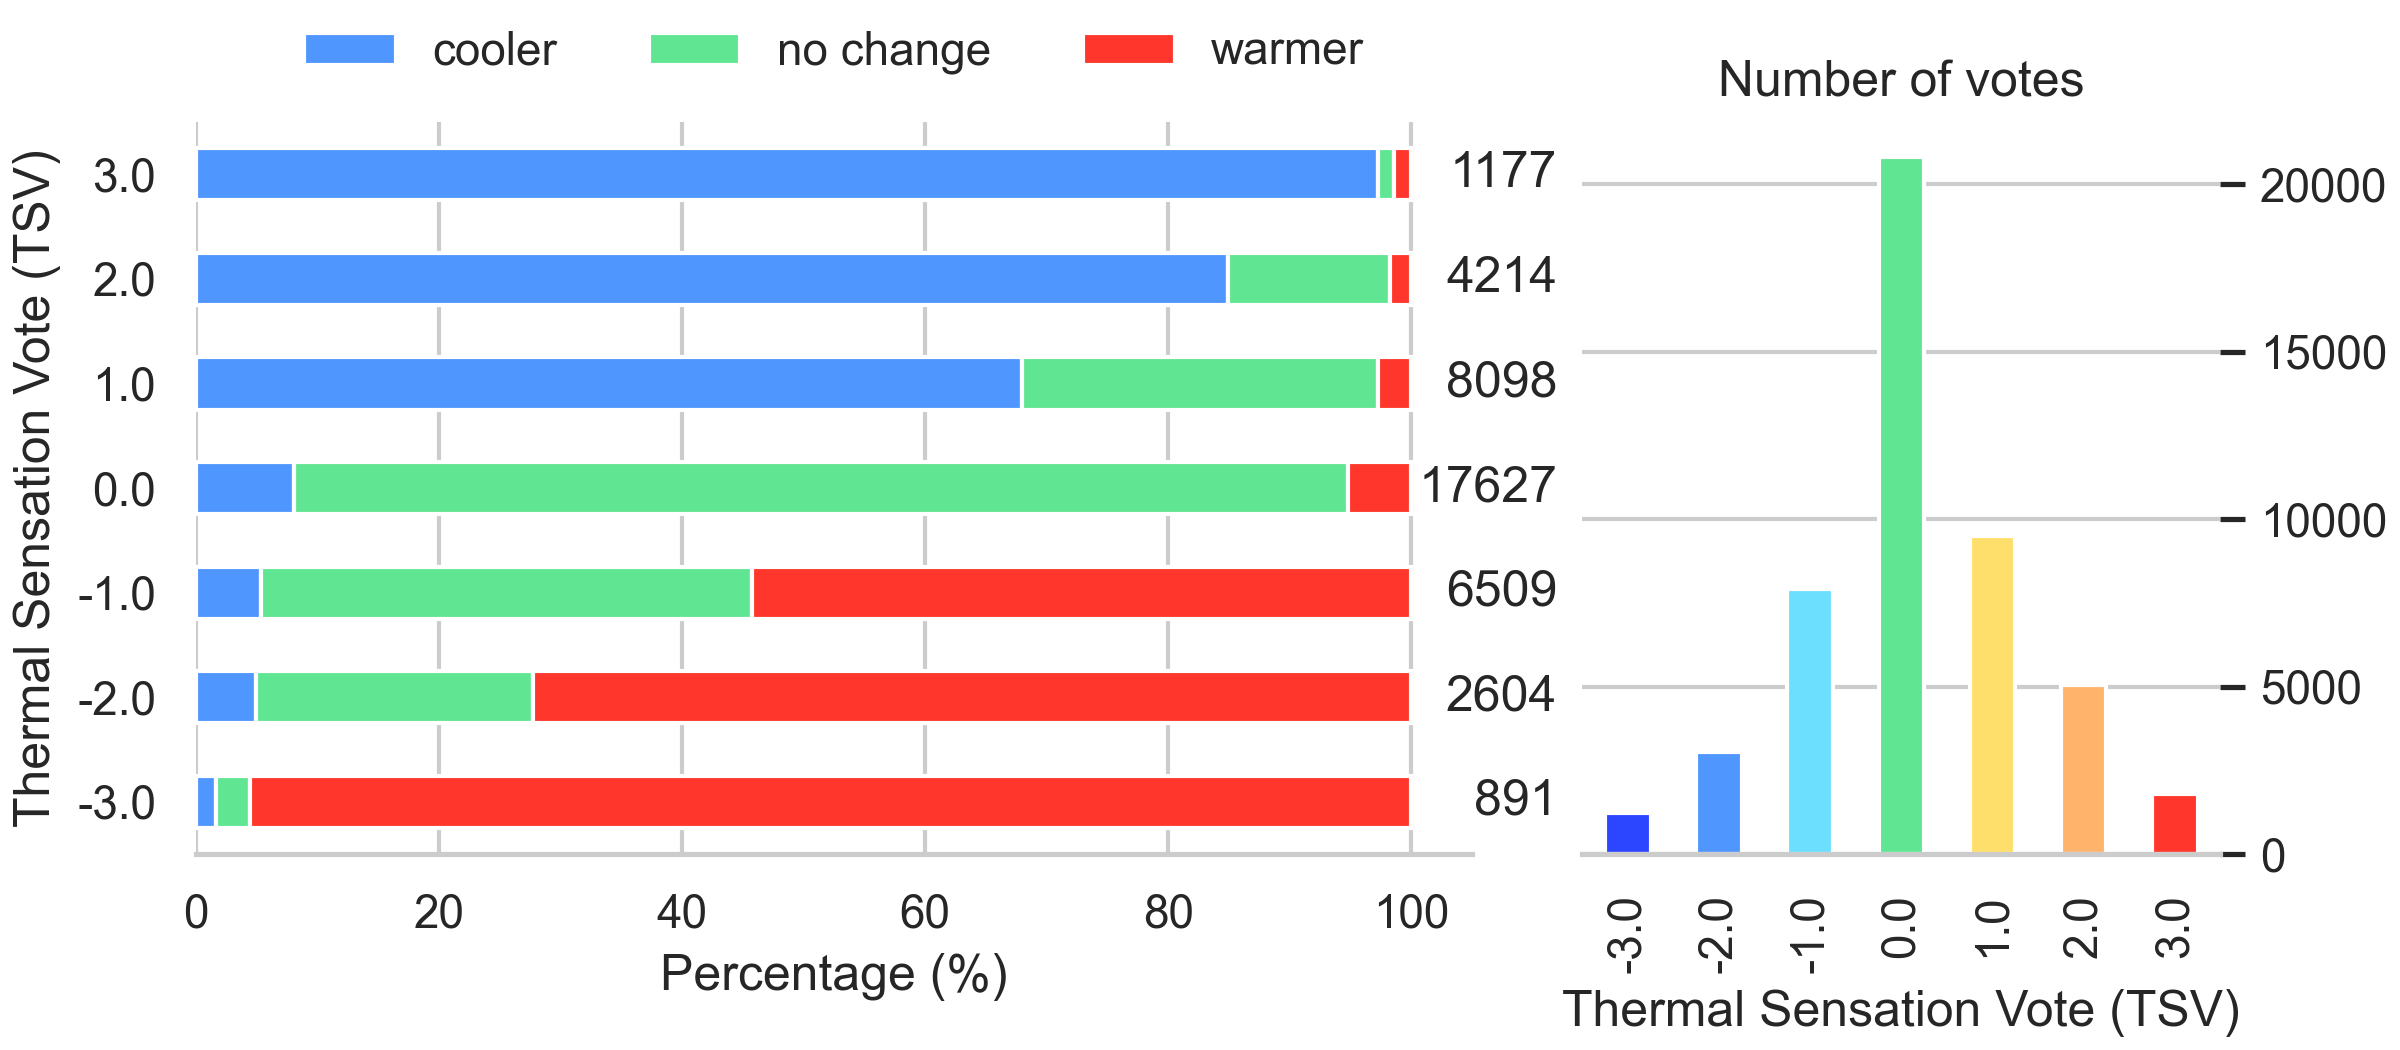
\includegraphics[width=\textwidth]{figures/bar_plot_tp_by_ts}
    \caption{The left Figure shows the percentage of \ac{tpv} for each thermal sensation vote.
    The numbers on the right side of each bar show the number of points for each \ac{tsv}.
    The right figure shows the total number of data points grouped by \ac{tsv}.
    Each bin in the right figure has more data points than in the left figure since less data on \ac{tpv} were available.}
    \label{fig:bar_plot_tp_by_ts}
\end{figure*}

In thermal comfort research, it is generally assumed that people who are `slightly warm' or `slightly cool' are thermally comfortable.
However, in the \ac{db2} \qty{68}{\percent} of participants who were `slightly warm' wanted to be `cooler' and \qty{54}{\percent} of participants who were `slightly cool' wanted to be `warmer'.
This finding challenges the above assumption.
Assuming that people who are `slightly warm' or `slightly cool' are comfortable leads to under-counting thermal discomfort in this example.
On the other hand, some participants who reported to be `cool', `cold', `warm', or `hot' wanted `no change'.
Of those who reported to be `cool' \qty{23}{\percent} of them wanted `no change' and \qty{5}{\percent} wanted to be `cooler'.
Similarly, but in reverse, among those who reported to be `warm' \qty{13}{\percent} wanted `no change' and \qty{2}{\percent} wanted to be `warmer'.
This result highlights one of the major limitations of the \ac{tsv} scale and of the assumption that people who are `slightly warm' or `slightly cool' are thermally comfortable.
This suggests that the thermal preference scale is better suited to determine how people perceive their thermal environment.
The \ac{tpv} more clearly allows an HVAC system to decide whether to change or not the thermal environment. 
On the contrary, the \ac{tsv} is ambiguous and does not allow determining if an action should be taken to increase the participant's thermal comfort.

\subsection{Comparison of PMV accuracy in predicting thermal sensation}\label{subsec:model-accuracy-comparison-in-predicting-thermal-sensation}
The \ac{pmv} was developed with the primary aim of predicting \ac{tsv}, consequently, we are here comparing the prediction accuracy of the two formulations.
The two models only differ when \ac{v} exceeds \qty{0.1}{\m\per\s};
hence we are also presenting the results for a subset of the data where \ac{v} is higher than \qty{0.2}{\m\per\s} since above this value the differences in the outputs of the two models are more pronounced.
We set the limit to \qty{0.2}{\m\per\s} and not a higher value since, as previously shown in Figure~\ref{fig:dist_input_data}, we could only reliably test the accuracy of the models up to \ac{v} of \var{v_95_perc_max}.
We did not use \qty{0.1}{\m\per\s} as a threshold because the original difference between the two models was \qty{0.2}{\m\per\s}.
The effect of air movement is perceptible only when the airspeed is sufficiently high to disrupt the body's thermal plume~\cite{zukowska_impact_2012}.
The threshold in the ASHRAE standard was reduced to \qty{0.1}{\m\per\s} to simplify the usability and achieve one threshold for all the air speeds.
% todo:
%  call charts a,b,c,d
\begin{figure*}[htb!]
    \centering
    \begin{subfigure}[b]{\textwidth}
        \centering
        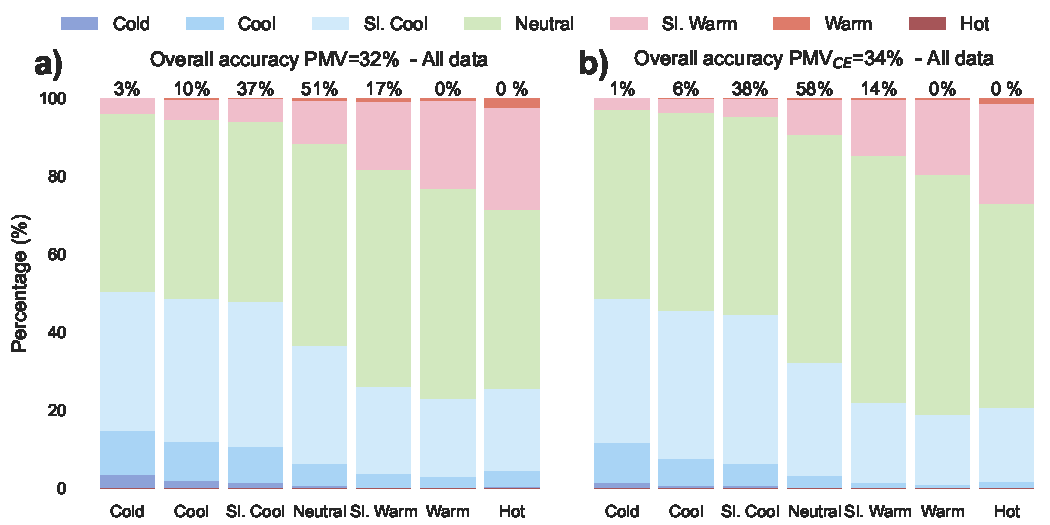
\includegraphics[width=\textwidth]{figures/bar_stacked_model_accuracy_0}
        \caption{All data}
     \end{subfigure}
    \begin{subfigure}[b]{\textwidth}
        \centering
        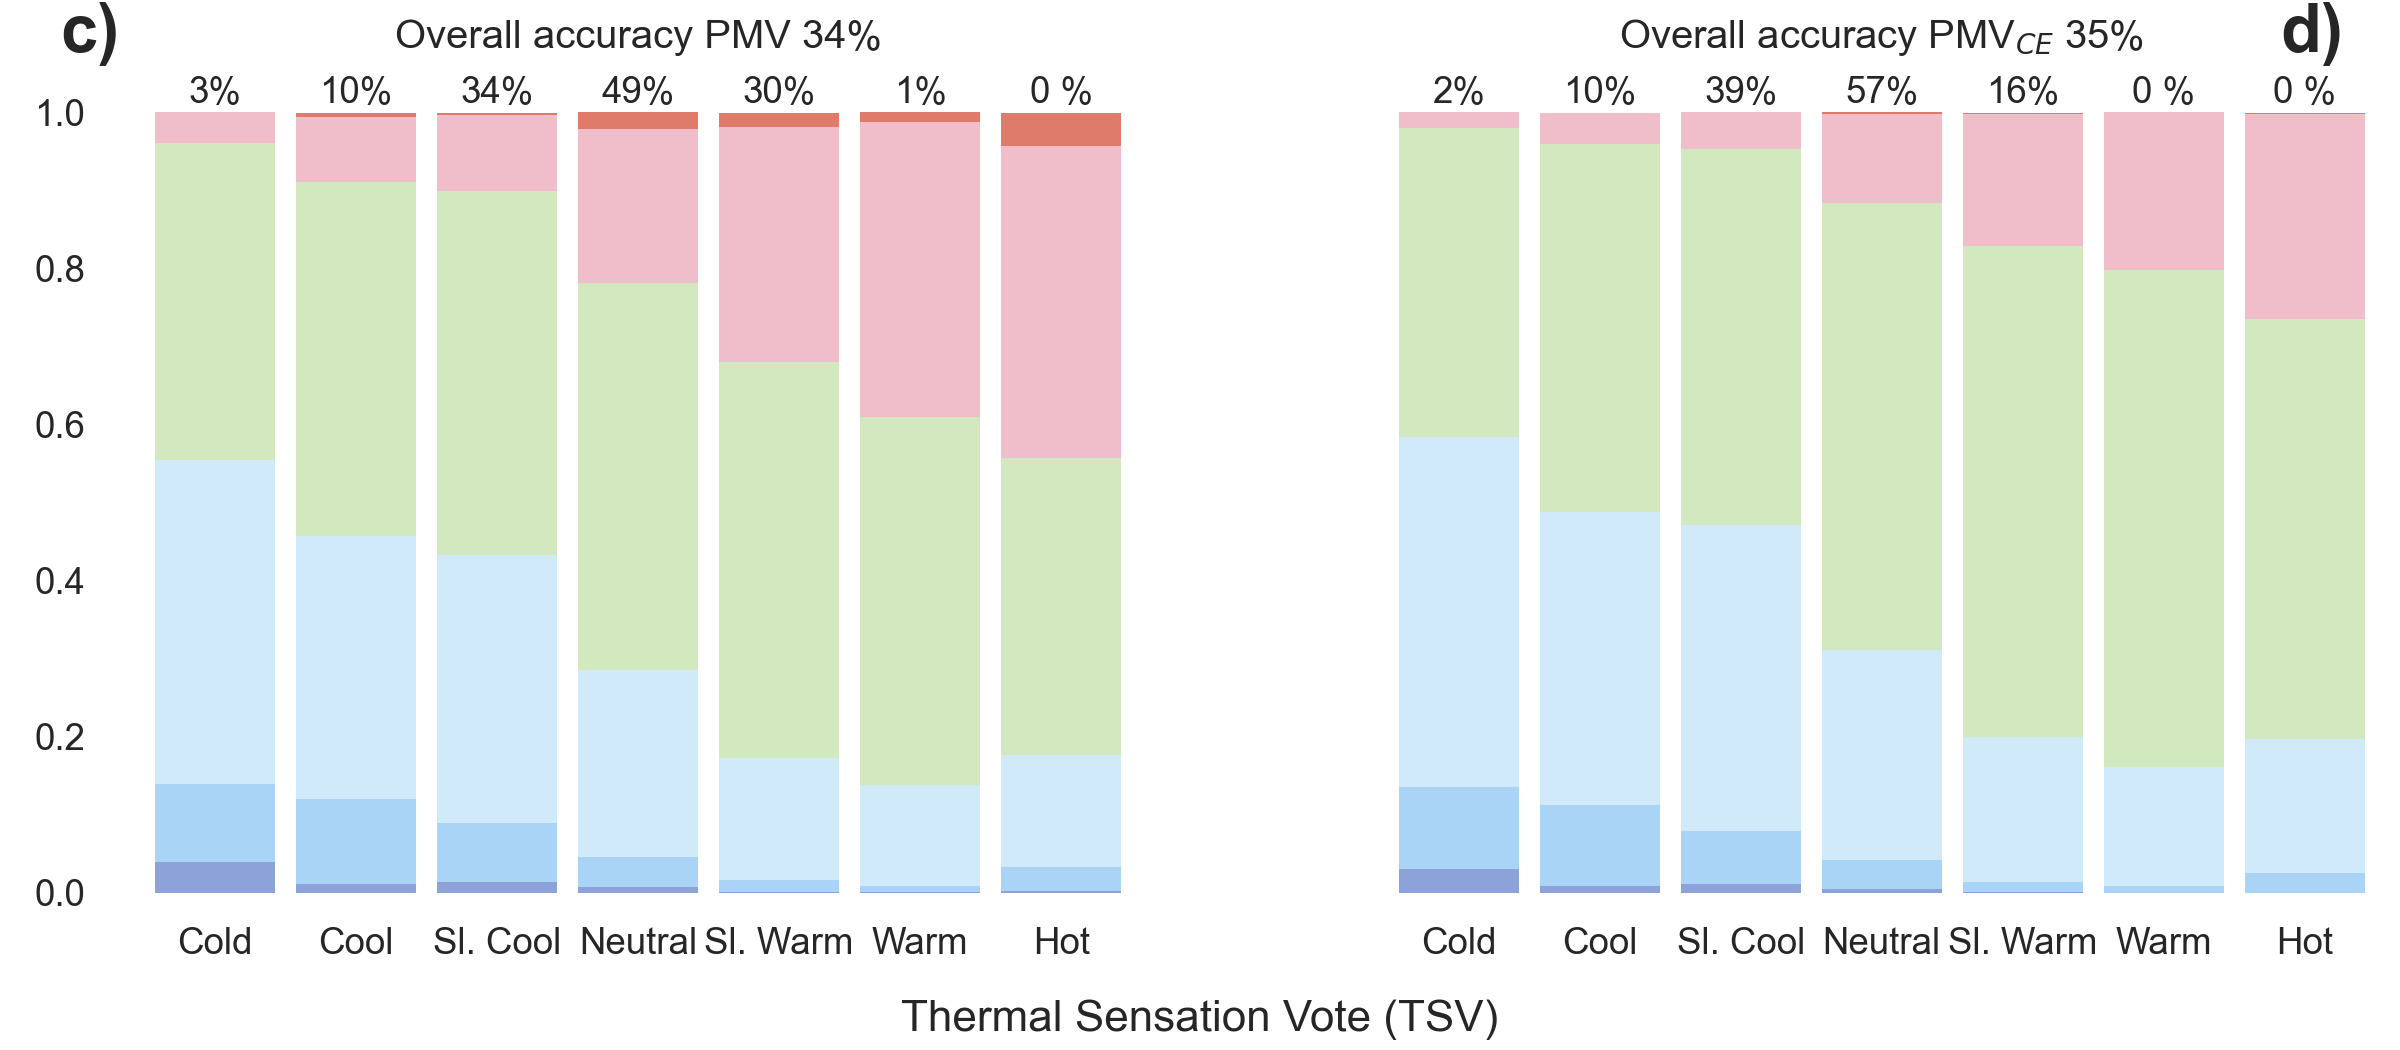
\includegraphics[width=\textwidth]{figures/bar_stacked_model_accuracy_0.2}
        \caption{Only data with \ac{v} $\geq$ \qty{0.2}{\m\per\s}}
     \end{subfigure}
    \caption{The calculated \ac{pmv} value is grouped by the \ac{tsv} value reported by the participants. 
    The number of data points in each bin of the two charts is the same and this allows us to compare the accuracy of both models.
    The overall prediction accuracy is shown above the chart while the model accuracy of predicting participants grouped by their \ac{tsv} is overlayed over each bar. 
    A random model, randomly selecting a thermal sensation vote would have an overall accuracy of \qty{14}{\percent}.}
    \label{fig:bar_stacked_model_accuracy}
\end{figure*}
Being \ac{tsv} the value reported by participants (i.e., ground truth), in Figure~\ref{fig:bar_stacked_model_accuracy} we grouped participants' responses by \ac{tsv} and reported the simple accuracy of the different \ac{pmv} formulations over each sub-figure.
Both \ac{pmv} formulations underestimated the conditions at which participants are thermally dissatisfied with their environment.
The overall accuracy of the \ac{pmv} and \ac{pmv-ce} were \qty{33}{\percent} and \qty{34}{\percent}, respectively.
Being the classification problem unbalanced, the simple accuracy is not an optimal metric to rate the model prediction accuracy since a default strategy of guessing the majority class would lead to a high overall model accuracy.
% todo describe the results for V>0.2
A model that would have always predicted `neutral' would have achieved an overall accuracy of \var{perc_tsv_neutral}, the number of participants who voted \ac{tsv}=0.
For this reason, in Table~\ref{tab:f1}, we report the F1-scores for all the models.
The F1-macro score, which is free from label imbalance, depicts that the accuracy of both models across all metrics is marginally better than random guessing (i.e., \qty{14}{\percent}).
\begin{table}[htb!]
    \centering
    \begin{tabular}{lccc}
\toprule
F1 score & PMV & PMV$_{CE}$ & Dataset \\
\midrule
 micro & 0.32 & 0.34 & \multirow{3}{*}{All data} \\
macro & 0.16 & 0.15 &  \\
weighted & 0.29 & 0.30 &  \\
\specialrule{.01em}{.05em}{.05em} micro & 0.32 & 0.35 & \multirow{3}{*}{\ac{vr} $\geq$ \qty{0.2}{\m\per\s}} \\
macro & 0.17 & 0.17 &  \\
weighted & 0.30 & 0.31 &  \\
\specialrule{.01em}{.05em}{.05em} micro & 0.30 & 0.31 & \multirow{3}{*}{\ac{vr} $\geq$ \qty{0.2}{\m\per\s} at three heights} \\
macro & 0.17 & 0.16 &  \\
weighted & 0.27 & 0.27 &  \\
\specialrule{.01em}{.05em}{.05em} micro & 0.43 & 0.45 & \multirow{3}{*}{$\lvert \textrm{PMV}\lvert \leq 1.5$ and $\lvert \textrm{TSV}\lvert \leq 1.5$} \\
macro & 0.23 & 0.22 &  \\
weighted & 0.42 & 0.43 &  \\
\bottomrule
\end{tabular}

    \caption{F1-score for the \ac{pmv} and \ac{pmv-ce} models.}
    \label{tab:f1}
\end{table}

% todo describe the table results
The \ac{pmv-ce} was specifically developed to more accurately estimate latent and sensible heat losses from the skin to the environment when air movement is used~\cite{arens_moving_2009}.
Both models had an accuracy lower than \qty{1}{\percent} when predicting either `warm', `hot', or `cold'.
This value is significantly lower and worse than random guessing, this is very concerning because this means that the models are actively misleading the users.
The low prediction accuracy of both model formulations, coupled with the lack of data in the extremes of the applicability limits of the models, may suggest that the models' applicability limits should be revisited.
% todo call it Standards implications, limit use PMV and of environmental variables
Based on our results we recommend restricting the use of the \ac{pmv} only to a values $\lvert \textrm{PMV}\lvert \leq 1.5$.
In addition, we also recommend restricting the ranges on both environmental and personal factors set by both \gls{55} and \gls{7730} Standards.
Currently, these limits extend far beyond the range of data contained in the \ac{db2} dataset.
Being the \ac{db2} the largest thermal comfort dataset in the world and containing data from all continents we deem not to be necessary to have such wide applicability limits for both \gls{55} and \gls{7730} Standards when these environmental variables are rarely observed in buildings across the world.
In addition, the lack of data available beyond the ranges depicted in Figure~\ref{fig:dist_input_data} did not allow us to test the accuracy of both the \ac{pmv} and \ac{pmv-ce} above those ranges.
Consequently, we suggest reducing both Standards applicability limits to the ranges shown in Table~\ref{tab:ranges}, until more data are collected.
\begin{table}[htb!]
    \centering
    \begin{tabular}{cc}
        \toprule
        Variable & Proposed range \\
        \midrule
        \ac{tdb} & \qtyrange{17}{30}{\celsius} \\
        \ac{tr} & \qtyrange{17}{30}{\celsius} \\
        \ac{rh} & \qtyrange{20}{80}{\percent} \\
        \ac{clo} & \qtyrange{0.3}{1.5}{clo} \\
        \ac{met} & \qtyrange{1}{2}{met} \\
        \ac{pmv} & \qtyrange{-1.5}{1.5}{} \\
        % todo shall we also include limits on Age?
        % todo shall we also include airspeed?
        \bottomrule
    \end{tabular}
    \caption{New proposed applicability limits for the \gls{55} and \gls{7730} Standards.}
    \label{tab:ranges}
\end{table}
Grouping the results into discrete categories introduces rounding errors since some participants reported \ac{tsv} on a continuous scale and the \ac{pmv} value is a continuous variable.
To compensate for this we plotted the \ac{pmv} and \ac{pmv-ce} values as a function of \ac{tsv} in Figure~\ref{fig:bubble_models_vs_tsv} and we plotted a \ac{lowess} curve.
\begin{figure*}[htb!]
    \centering
    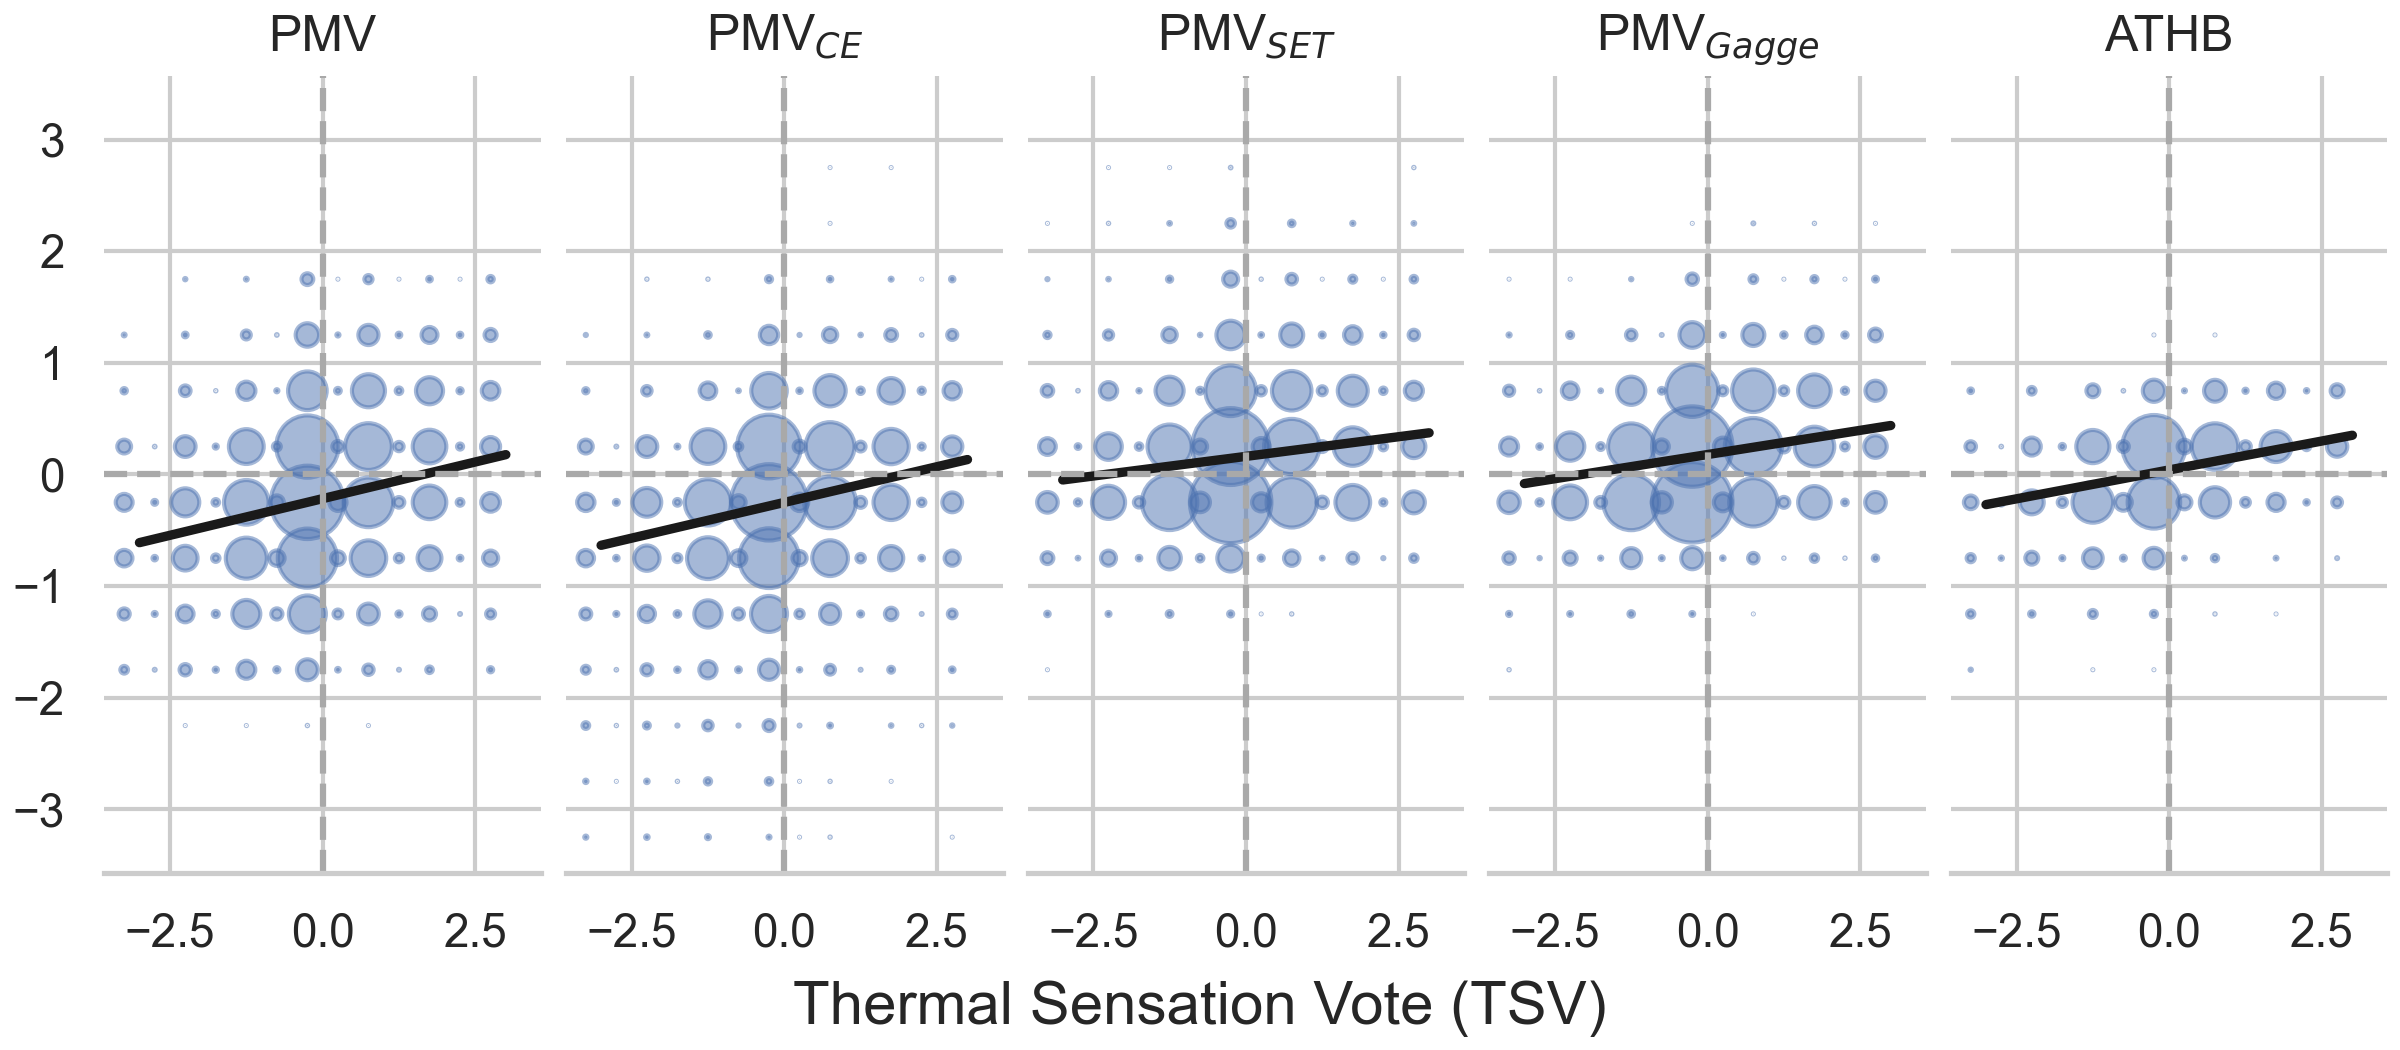
\includegraphics[width=\textwidth]{figures/bubble_models_vs_tsv}
    \caption{The \ac{lowess} curve shows the relationship between the raw \ac{pmv} and \ac{tsv} data.
    Raw data were then binned and a bubble chart (circle area is proportional to the number of votes in that bin) is superimposed over the regression curve to aid the visualization of a large dataset.}
    \label{fig:bubble_models_vs_tsv}
\end{figure*}
The curve, in the Figure, is calculated using the individual data and not the binned data.
We binned the data to aid the visualization of a large dataset.
If the model is to accurately predict the thermal sensation of people, the regression line should pass through the origin of the cartesian plane and have a slope of 1.
The intercepts for the \ac{pmv} is \qty{-0.23} and for the \ac{pmv-ce} is \qty{-0.24} which means that the model has a bias of less than one-quarter of a thermal sensation interval. 
The intercept is close to 0 and this is aligned with the results shown above that the model can predict people who reported to be neutral \qty{55}{\percent} and \qty{58}{\percent} of the times.
Both \ac{pmv} formulations always underpredicted the thermal sensation of people who reported to be on the extremes of the \ac{tsv}; the slope of the curve was significantly lower than 1.
We discuss in detail in sub-Section~\ref{subsec:sources-of-error} which factors may be the underlying cause of these errors.

The intended aim of the \ac{pmv} model is not to accurately predict each individual thermal response from participants.
The \ac{pmv} model was developed to predict the average thermal sensation of an undefined large group of occupants sharing the same environment.
Consequently, while the above-mentioned analysis is needed to compare for the same sample size in each thermal sensation group the \ac{pmv} and \ac{pmv-ce} accuracies, it focuses primarily on comparing individual \ac{tsv} to \ac{pmv}.
This type of analysis does not conclusively disprove the inefficacy of the \ac{pmv} models in predicting the average thermal sensation of a large group of occupants.
This was already done in \mycite{Cheung2019}, where they grouped people based on the same heat loss or gains (same \ac{pmv} ranges), not the same thermal sensation vote as we did here, and then quantified how many times the \ac{pmv} model correctly predicted \ac{tsv}.
They found that the accuracy of \ac{pmv} in predicting \ac{tsv} was only \qty{34}{\percent} \mycite{Cheung2019}. 

\subsection{Model Bias}\label{sec:model-bias}
\subsubsection{Model Overall Bias}\label{subsec:model-overall-bias}
We calculated the overall bias of the model as previously done by \mycite{Humphreys2002} by subtracting the \ac{pmv} and  \ac{pmv-ce} models prediction from the self-reported \ac{tsv}.
Results are presented in Figure~\ref{fig:hist_discrepancies}.
% todo:
%  describe in the paper that we used test to determine that data are not normally distributed.
%  We cannot change into a letter value plot since in that case it would be hard to highlight the number of responses that are within the range from -.5 to.5.
%  The Caption is missing
\begin{figure*}[htb!]
    \centering
    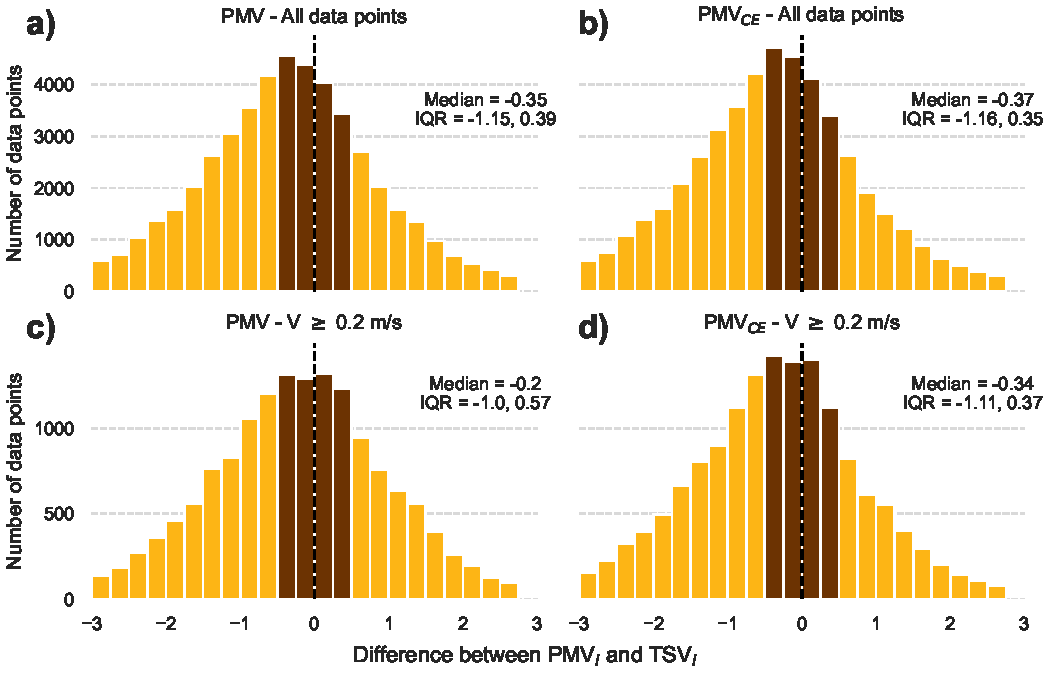
\includegraphics[width=\textwidth]{figures/hist_discrepancies}
    \caption{}
    \label{fig:hist_discrepancies}
\end{figure*} 
Overall both the \ac{pmv} and \ac{pmv-ce} models have a median bias lower than half of a thermal sensation interval.
Figure~\ref{fig:hist_discrepancies} contains the summary statistics, and the results highlight that the \ac{pmv-ce} had a higher bias than the \ac{pmv} when using the entire dataset.
The results show that the median bias of the \ac{pmv} model reduced to \var{bias_median_pmv_0.2} from \var{bias_median_pmv_0}, meaning that at higher speed the \ac{pmv} model improved.
Surprisingly, we found that the median bias for the \ac{pmv-ce} increased to \var{bias_median_pmv_ce_0.2} from \var{bias_median_pmv_ce_0}.
These are worrying results since the \ac{pmv-ce} model claims to have a higher accuracy at higher values of \ac{v}, but this is not what was found from this data.
As far as we could find, there is no published paper proving a higher accuracy of the \ac{pmv-ce} compared to the \ac{pmv} model. 
The \ac{pmv-ce} has lower accuracy while making the code more complex and computationally intensive to run.

\subsubsection{Model Bias as Function of Four Input Variables}\label{subsec:model-bias-variable}
In the previous section, we presented the overall bias of the two \ac{pmv} formulations.
We then went on to determine how the bias varied as a function of \ac{tdb}, \ac{v}, \ac{met}, and \ac{clo}.
% todo add humidity ratio chart
We did not include \ac{tr} in the analysis since \ac{tr} was not reported in several studies, hence, we estimated it as detailed in the Methodology.
Furthermore, in many buildings is possible to assume \ac{tr} equal to \ac{tdb} without committing a major error~\cite{Dawe2020}.
Figure~\ref{fig:dist_input_data} shows the results.
In each sub-figure, we have binned the results into discrete intervals of equal width, and the x-axis tick label is the center value of the interval.
All the violin plots have the same area to aid visualization, despite the fact that the number of points in each bin is not constant.
% todo:
%  I need to have the red lines for the same inverse reason why I cannot use the boxenplot in the previous chart

\begin{figure*}[htb!]
    \centering
    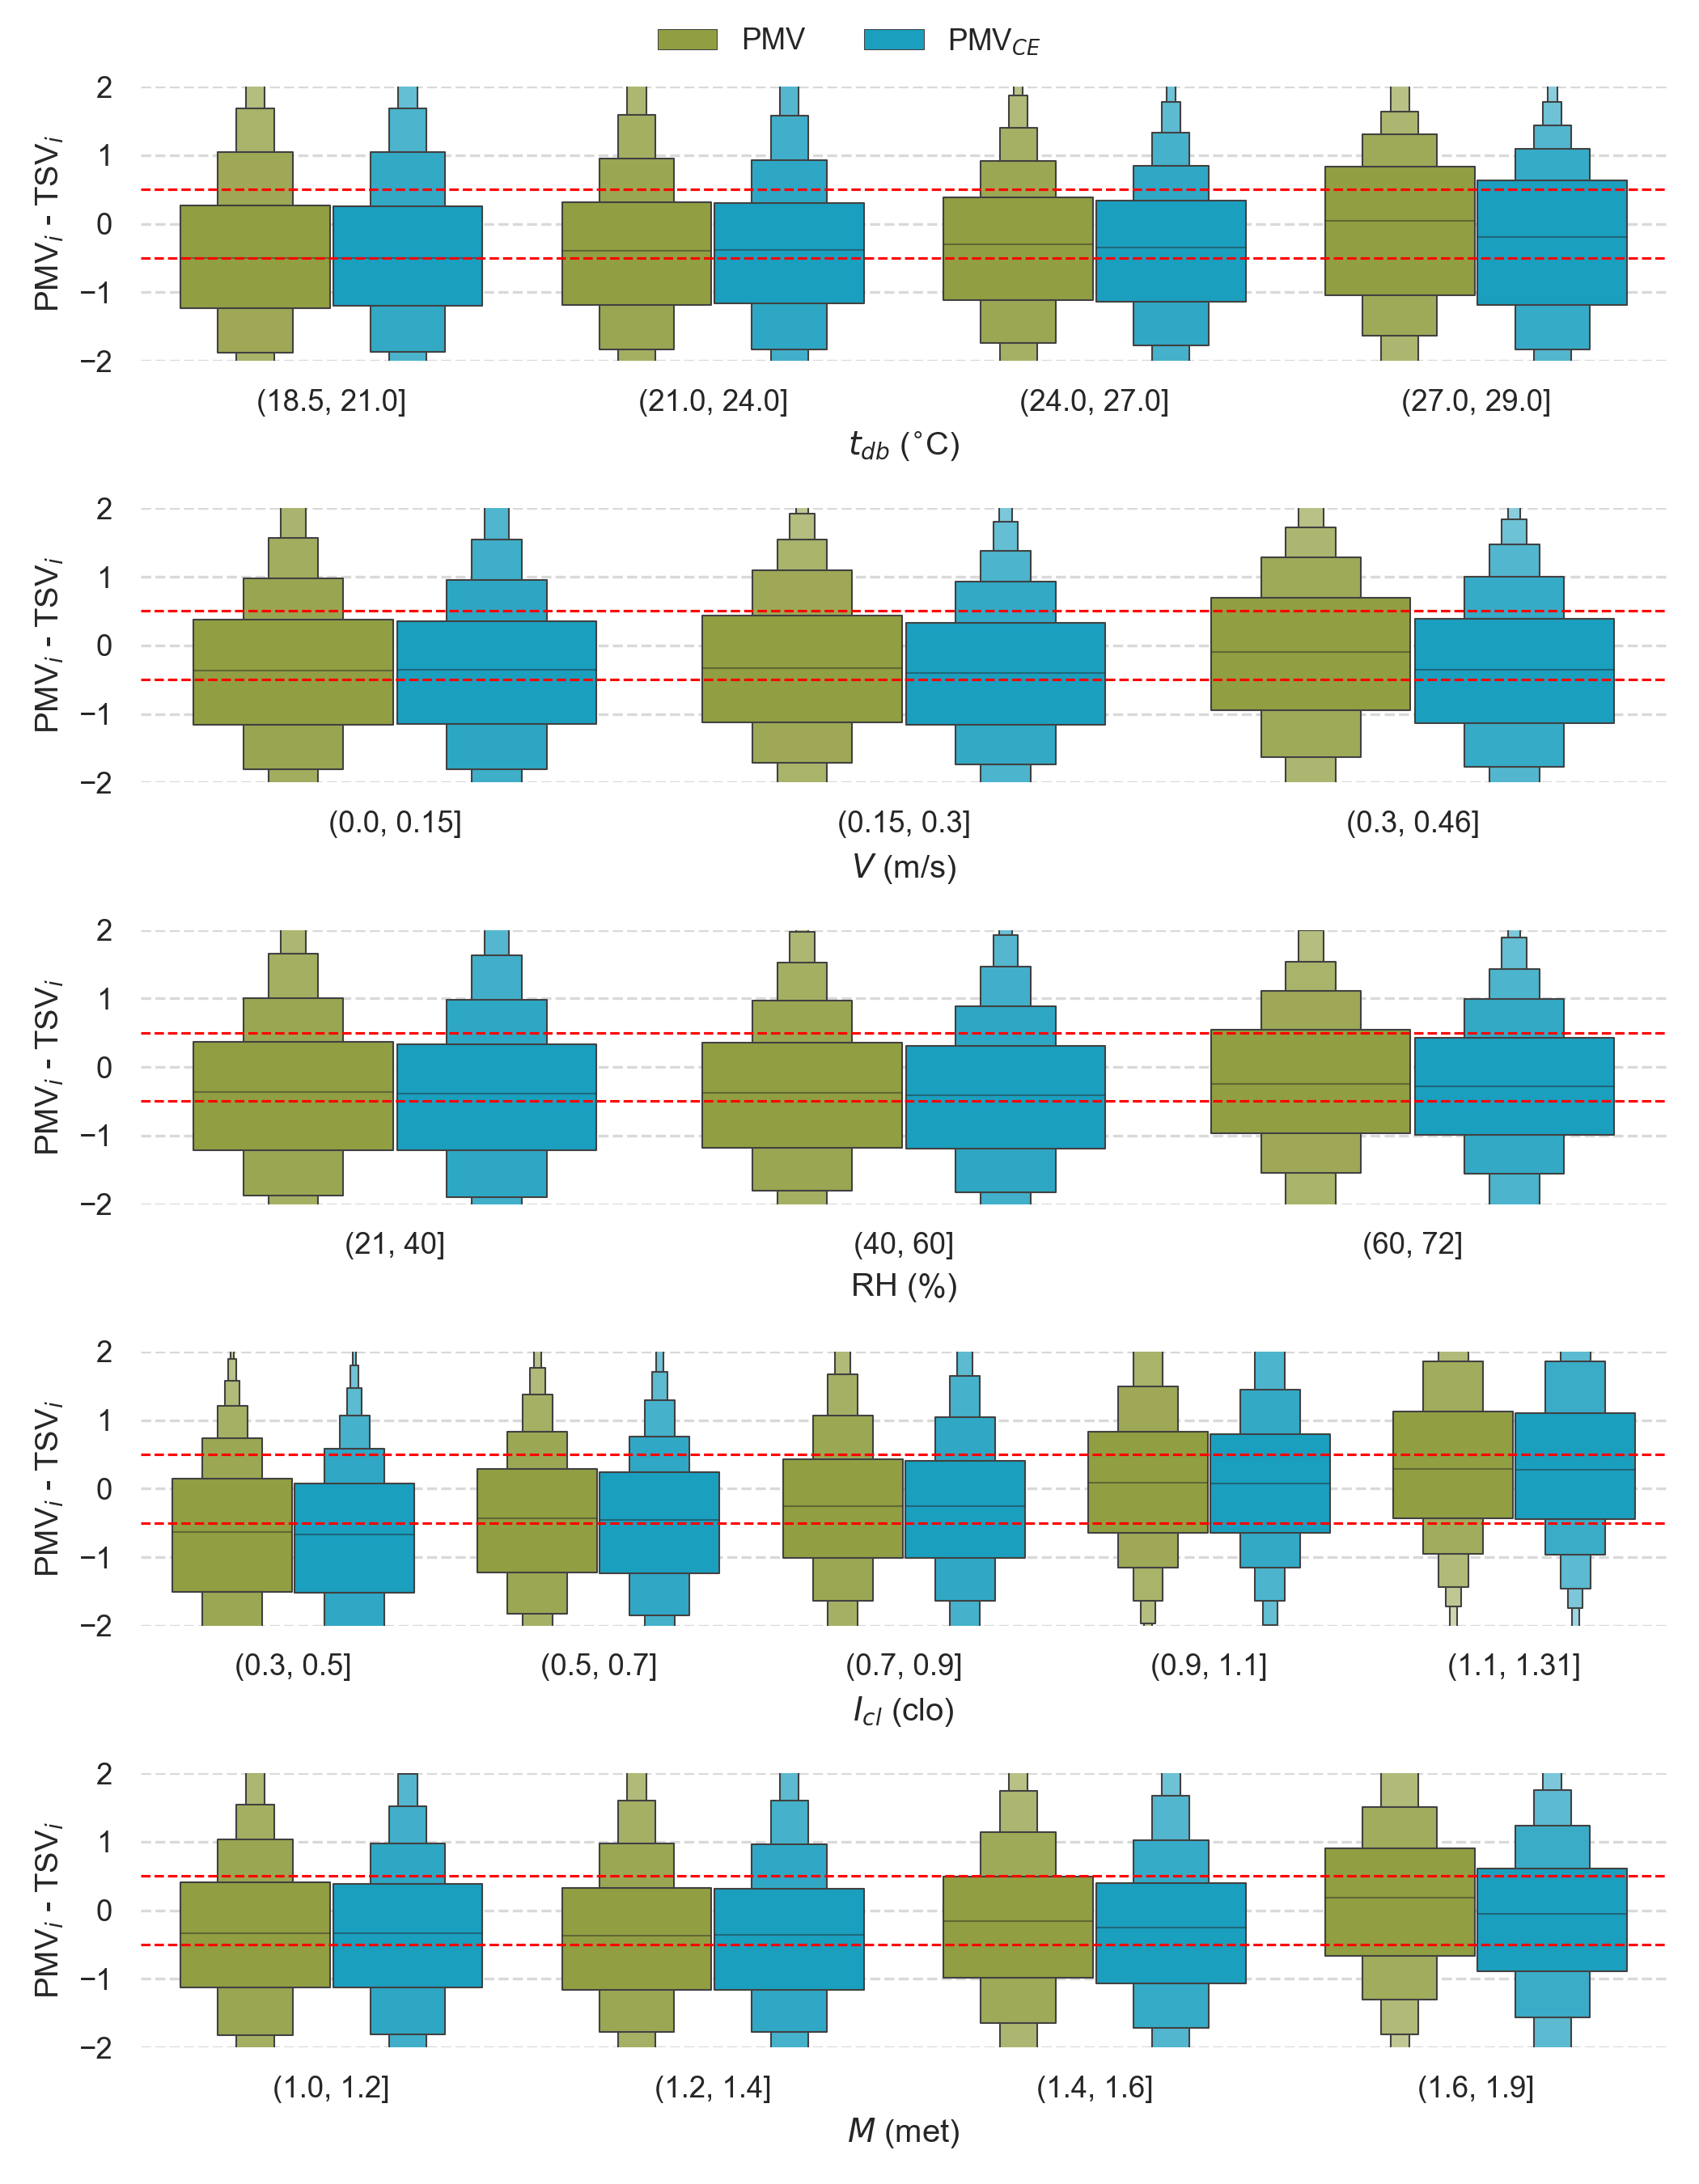
\includegraphics[width=\textwidth]{figures/bias_models}
    \caption{Bias of the \ac{pmv} and \ac{pmv-ce} models plotted as a function of the input variables.}
    \label{fig:bias_models}
\end{figure*}
The results depict that the use of the \ac{pmv-ce} model did not improve the bias of the \ac{pmv} results across all four input variables.
On the contrary, the bias of the \ac{pmv-ce} diverged more from 0 as the value of \ac{v} increased.
These results are in agreement with those presented in the previous section and depict that the correction applied by the \ac{pmv-ce} model worsens the results. 

\subsection{Comparison between the PMV formulations with the two-node model}\label{subsec:comparison-between-the-pmv-formulations-wih-the-two-node-model}
% todo consider moving to appendix and explain well why I have done this.
We compared how the results of the \ac{pmv} and \ac{pmv-ce} perform against the results of the two-node model because xxxx.
Figure~\ref{fig:pmv_two_node_comparison} was generated by calculating the three \ac{pmv} values using the same combination of \num{10000} randomly generated sets inputs.
The \ac{pmv} and \ac{pmv-ce} were then plotted on the y-axis while the \ac{pmvg} value was on the x-axis.
The Figure also shows the \ac{lowess} curves that are used to visualize the prevailing data trend.
The results of the \ac{pmv} model had a higher agreement than those obtained with the \ac{pmv-ce} model for \ac{pmvg} $\geq$ \qty{0.5}{\m\per\s}.
These results show the \ac{pmv-ce} is less similar to the \ac{pmvg} model than the \ac{pmv}, despite using it in the backend to calculate the cooling effect.
This is also an unexpected result and we will discuss why this may be in the following paragraph. 
% todo When a figure report how well a variable is predicted, for example x-measured vs x-predicted, the graph must be a square, otherwise it is visually skewed. 1) I suggest to use the words instead of numbers for PMV 2) We should be consistent with the PMV naming we used (do not use ASHRAE and ISO here) 3) why both models are far from Gagge for PMV<0, both model in general produce a cooler feeling than PMVgagge, we should explain why if we keep this paper. 

\begin{figure*}[htb!]
    \centering
    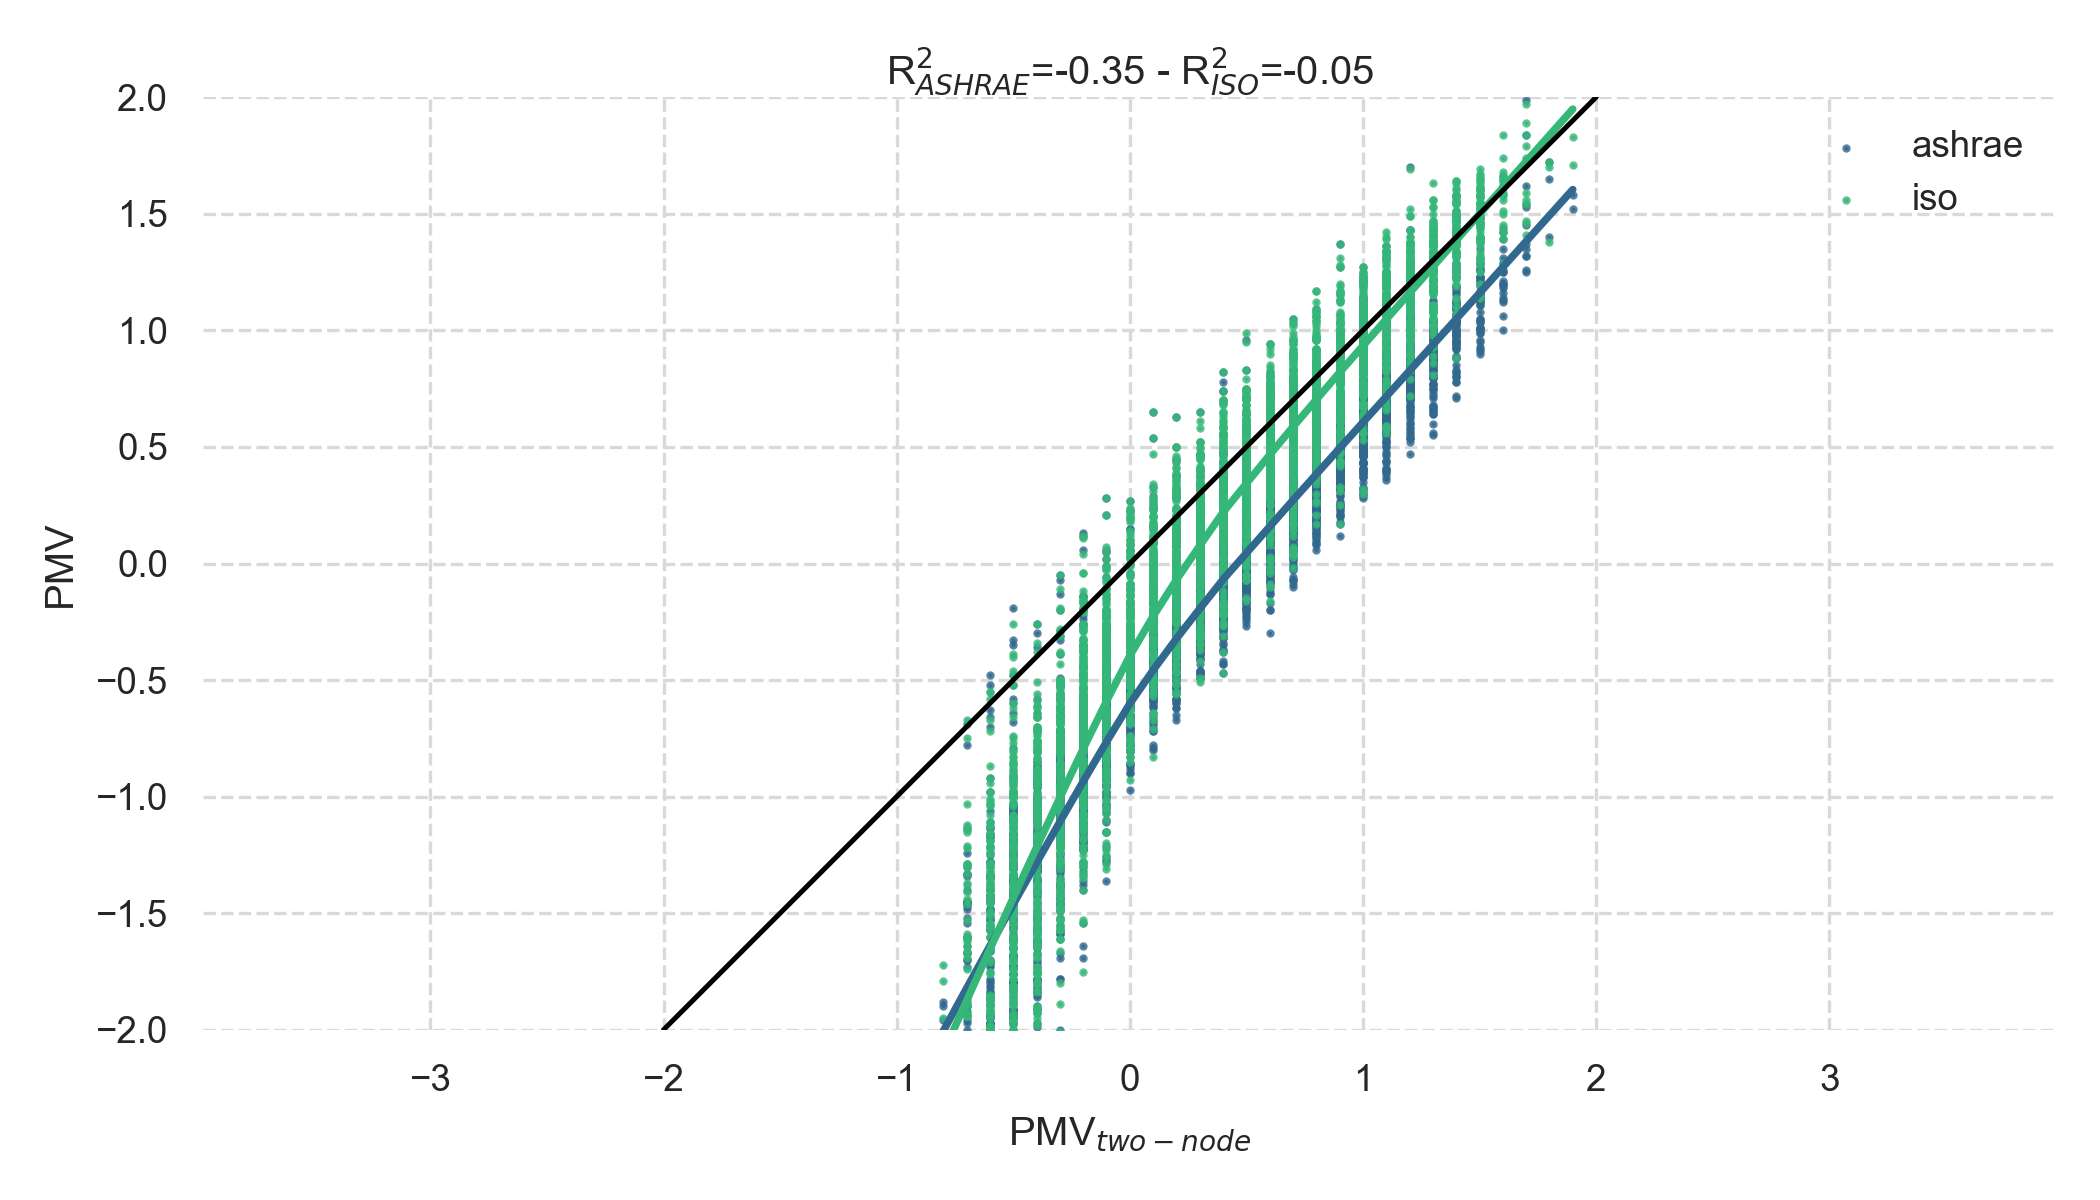
\includegraphics[width=\textwidth]{figures/pmv_two_node_comparison}
    \caption{}
    \label{fig:pmv_two_node_comparison}
\end{figure*}

\subsection{Sources of Error}\label{subsec:sources-of-error}
In this Section, we identify some of the main reasons that could explain the difference in the results from the two \ac{pmv} models when compared against the \ac{tsv} available in the \ac{db2}.
Moreover, we tried to explain why we observed that the \ac{pmv-ce} model has a lower accuracy than the \ac{pmv} in predicting thermal sensation.
The issues are reported in order of importance of what we believe may affect the accuracy of the model.
More research is needed to determine how to improve the overall accuracy of the \ac{pmv} model.

\paragraph{Heat Balance Equation and Calculation of the PMV value}
The \ac{pmv} model uses simplified heat balance equations to estimate the heat loss and gains from the human body to its surrounding environment.
This is a possible source of error since the model considers the human body to be a cylinder with constant width all uniformly covered with clothing where the heat is all generated in its core.
This is a great simplification since it ignores, for example, the fact that different parts of the body may not be covered by clothing, the metabolic heat generation is not uniform, the mass-to-surface ratios are not constant, and it ignores vasoconstriction and vasodilation.
However, the \ac{pmv} model erroneously assumes that the human body, aside from some edge cases, is either losing or gaining heat from its surrounding environment.
This is not the case, since the human body in most conditions observed indoors activates control strategies to maintain a constant core temperature.
Moreover, the \ac{pmv} model has been developed based on the assumption of steady-state heat transfer, however, this never precisely occurs since the human thermoregulatory system is always actively engaged to ensure a stable core temperature.

The \ac{pmv} model uses the overall heat losses or gains, which are only a proxy to the thermal stress that the human body has to undergo to maintain a constant internal temperature, to a \ac{pmv} value which should represent a \ac{tsv} vote.
Fanger created this equation based on a few experimental data collected in a laboratory, and despite the growing body of literature, this equation was never updated~\cite{Fanger1970}.
In the \ac{pmv} model the heat losses and gains are mapped using constant coefficients to a thermal sensation vote, disregarding the fact that the human body does not have the same ability to compensate for warm and cold conditions.

It is, therefore, not surprising to observe that the \ac{pmv} model has an `acceptable' accuracy in determining when people are `neutral`.
This is equivalent to no heat losses or gains (i.e., \ac{pmv}=0) which means that the body is dissipating all the internal metabolic heat production through conduction, convection, or radiation without needing to thermoregulate using sweating, shivering, vasoconstriction, vasodilation, behavioral adjustments, and non-shivering thermogenesis.
On the other hand, the model cannot correctly predict the thermal sensation of people who report being outside the three central thermal sensation votes (slightly cool, neutral and slightly warm).
We showed that people tend to be closer to neutrality than what the models predicted (see figure XXX), this is an indication that they were exposed to compensable thermal conditions. Therefore, the models' inability to account for these regulatory mechanisms is a fundamental limitation.

To continue using the \ac{pmv} model beyond an absolute value of 1, more research is needed to determine whether the inaccuracy of the model is related to either or a combination of the following factors and if those sources of inaccuracy can be reduced: 
i) the assumption that the heat losses/gains estimated by the \ac{pmv} are correlated to the thermoregulatory response that the body has to undertake to compensate for unsatisfactory thermal comfort conditions;
ii) the correlation coefficients used by Fanger to link the heat losses/gains and thermal stress are constant and not xxx;
iii) the regression coefficient between heat losses and heat gains and thermal stress are not the same for the heat losses and gains and two different equations should be used;
iv) the anchors used by the \ac{pmv} model are different from those used by participants in reporting their thermal sensation.
For example, while the \ac{pmv} model may assume that a score of 3 (hot) signifies the change between a compensable set of conditions to an un-compensable one, e.g., their skin wettedness reaches the max value ($w_{max}$), as suggested by Gagge's in his manuscript~\cite{GaggeSET}.
Participants in commercial buildings may, on the contrary, deem the environment to be `Hot' as soon as they start sweating and their \ac{w} crosses a critical threshold which is only a fraction of $w_{max}$.

It is likely that a combination of all the above-mentioned factors plays a role in explaining the discrepancies between the \ac{pmv} model and the self-reported \ac{tsv}.
The fourth hypothesis has gained significant momentum in the literature which led to the development of several \ac{pmv} formulations that apply correction factors to the final \ac{pmv} result without changing the underlying equation~\cite{Yao2022, Toftum2002}

\paragraph{Measurement Errors}
All the data contained in the \ac{db2} have been published in peer-reviewed manuscripts, however, measurement errors are inevitably present in the dataset.
This is due to the fact that all measurement instrumentation is not always calibrated before use, the uncertainty of the measurements may be large, the placement of the instrumentation may not be in the near proximity of the participant, and estimating clothing and metabolic rates from tables is a complex and prone to error task.
In an ideal scenario, errors would be random and would cancel out, not significantly affecting the overall bias of the model but only affecting the standard deviation of the error~\cite{Humphreys2002}.
However, this may not always be the case, for example, if a researcher often underestimated the clothing insulation of participants or their activity levels.

\paragraph{Thermal Sensation Scale}
One minor but not negligible source of error is using a discrete scale to assess thermal sensation (most of the \ac{tsv} in the \ac{db2} were collected using a discrete scale) while the \ac{pmv} output is continuous.
For example, even if the model was 100~\% accurate and the estimated \ac{pmv} value was \num{2.5} the person could only report being `warm (+2)' or `hot (+3)'.
Using a continuous, may in principle be a more robust approach and align with the output but \mycite{schweiker2019scales} showed that the distances between the anchors are not constant ~\cite{schweiker2019scales, schweiker2020evaluating}. 
They also showed that the \ac{tsv}'s assumption of its independence from contextual factors such as climate, season and language is flawed~\cite{schweiker2019scales, schweiker2020evaluating}.
An alternative solution would be to transform the \ac{pmv} output to an ordinal and categorical seven-point scale. 

% \paragraph{Other neglected factors}
% Errors are also caused by the fact that the \ac{pmv} model is an approximation of a highly complex system (the human body and mind) that interacts with the surrounding environment.
% Fanger could not, therefore, include all the factors that contribute to the comfort vote and some of them have been omitted.

% todo write a paragraph trying to find the reason why the PMV CE model is less accurate.
% todo write a paragraph about what we recommend for ASHRAE 55